\section{Segregasi Tanggung Jawab Kueri dan Perintah}

Segregasi tanggung jawab kueri dan perintah (\textit{Command-Query Responsibility Segregation}, CQRS) merupakan sebuah pola yang memisahkan operasi baca dan tulis untuk sebuah media penyimpanan data. Dalam pemodelan data, seringkali model data yang sama digunakan untuk operasi pembacaan dan pembaruan. Meskipun begitu, seringkali kedua operasi tersebut memiliki kebutuhan yang berbeda. CQRS menggunakan model data yang berbeda untuk operasi yang berbeda. Selain itu, beban pekerjaan untuk kedua operasi tersebut seringkali asimetris dan memiliki kebutuhan kinerja dan penskalaan yang berbeda \parencite{msCQRS}.

Perintah (\textit{command}) merupakan pesan yang berfokus pada pekerjaan, seperti "pesan kamar hotel" dibandingkan dengan "ubah status reservasi suatu kamar menjadi sudah dipesan". Dengan pendekatan ini, perintah dapat diproses secara asinkron.

\begin{figure}[ht]
    \centering
    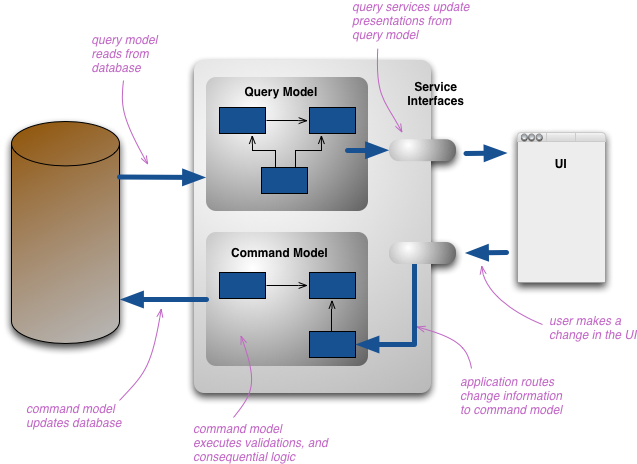
\includegraphics[width=0.8\textwidth]{resources/chapter-2/cqrs.png}
    \caption{Ilustrasi CQRS \parencite{fwCQRS}}
    \label{fig:cqrs-illustration}
\end{figure}

Pendekatan ini memungkinkan pemisahan data untuk operasi baca dan data untuk operasi tulis. Pembacaan data dapat dilakukan pada skema atau basis data yang telah dioptimalkan untuk operasi tersebut, seperti menyimpan data di memori, \textit{materialized view}, atau pun yang lainnya.

Pendekatan ini memungkinkan penskalaan secara independen dan \textit{separation of concerns}. Meskipun begitu, implementasinya bisa menjadi kompleks dan apabila basis data untuk operasi pembacaan dan penulisan berbeda, data menjadi \textit{eventual consistent}.